\documentclass[conference]{IEEEtran}
\IEEEoverridecommandlockouts

\usepackage{cite}
\usepackage{amsmath,amssymb,amsfonts}
\usepackage{graphicx}
\usepackage{textcomp}
\usepackage{xcolor}
\usepackage{makecell}
\usepackage{listings}
\usepackage{xurl}
\usepackage{hyperref}

\definecolor{codegreen}{rgb}{0,0.6,0}
\definecolor{codegray}{rgb}{0.5,0.5,0.5}
\definecolor{codepurple}{rgb}{0.58,0,0.82}
\definecolor{backcolour}{rgb}{0.95,0.95,0.92}

\lstdefinestyle{mystyle}{
    backgroundcolor=\color{backcolour},
    commentstyle=\color{codegreen},
    keywordstyle=\color{magenta},
    numberstyle=\tiny\color{codegray},
    stringstyle=\color{codepurple},
    basicstyle=\ttfamily\footnotesize,
    breakatwhitespace=false,
    breaklines=true,
    captionpos=b,
    keepspaces=true,
    numbers=left,
    numbersep=5pt,
    showspaces=false,
    showstringspaces=false,
    showtabs=false,
    tabsize=2
}
\lstset{style=mystyle}

\title{High-Precision Temperature Measurement using PT100}

\author{
    \IEEEauthorblockN{Puni Aditya, Vivek K Kumar and Dr. G.V.V. Sharma}
    \IEEEauthorblockA{Department of Electrical Engineering,
    \\Indian Institute of Technology Hyderabad,\\
    Kandi, India 502284
    \\ gadepall@ee.iith.ac.in}
}

\begin{document}
\maketitle

\begin{abstract}
This paper details the design, implementation, and validation of a temperature measurement system using a PT100 resistance temperature detector (RTD), a high-precision ADS1115 ADC, and an Arduino microcontroller. The system employs a differential voltage reading from a simple divider circuit for signal acquisition. A quadratic model, $V = aT^2 + bT + c$, was derived using the Least Squares method on a training dataset. This model was then validated against a separate, unseen dataset to verify its accuracy. The final calibrated temperature is displayed on a JHD 162A parallel LCD, creating a validated and accurate measurement device.
\end{abstract}

\section{Introduction}
Accurate temperature measurement is critical in various scientific and industrial applications. While many sensors exist, platinum resistance thermometers like the PT100 offer high accuracy and stability over a wide temperature range. However, their small resistance change necessitates precise measurement techniques. This project moves beyond the Arduino's internal ADC by interfacing with an external 16-bit ADS1115 ADC to achieve higher resolution. This paper presents the hardware setup, the software implementation, and the mathematical modeling used to calibrate the system for optimal accuracy.

\section{Hardware Setup}
The components used to construct the temperature measurement system are listed in Table \ref{table:list}. The complete circuit schematic is shown in Fig. \ref{fig:schematic}. The key connections for the ADC and LCD are detailed in Table \ref{table:ads_connections} and Table \ref{table:lcd_connections}.

\begin{figure}[!h]
    \centering
    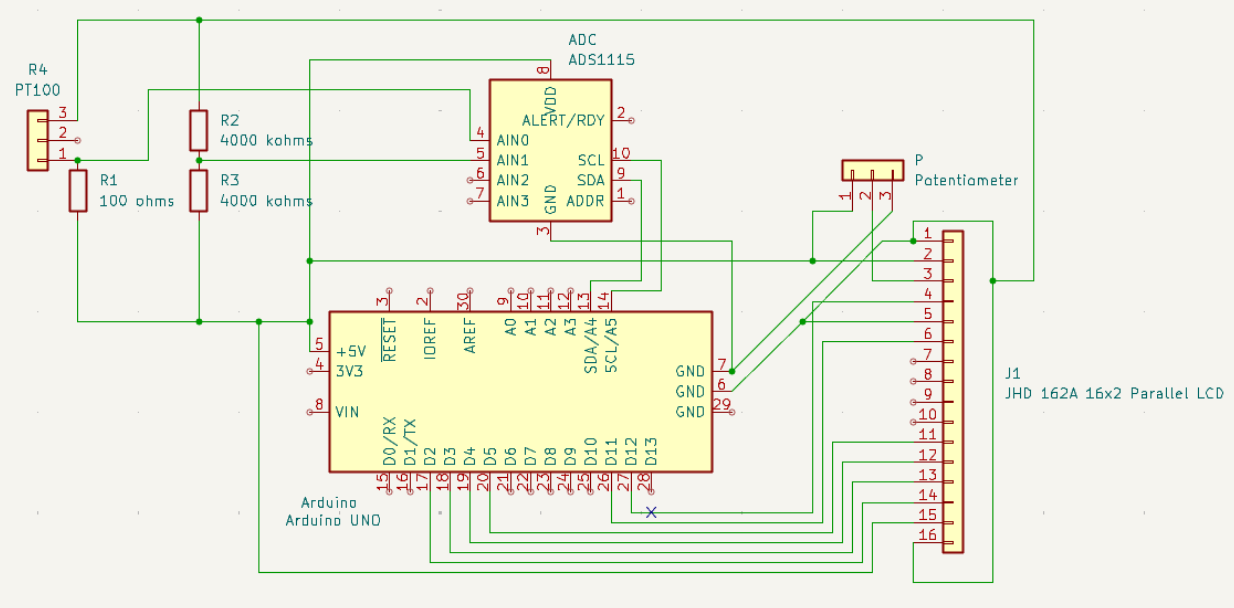
\includegraphics[width=\columnwidth]{figs/circuit_schematic.png}
    \caption{Circuit Schematic}
    \label{fig:schematic}
\end{figure}

\begin{table}[!h]
  \centering
  \caption{List of Components}
  \label{table:list}
  \begin{tabular}{|l|c|p{4cm}|}
    \hline
    \textbf{Component} & \textbf{Qty.} & \textbf{Description} \\
    \hline
    Arduino Uno & 1 & Microcontroller for processing and control. \\
    \hline
    ADS1115 ADC & 1 & 16-bit external ADC for high-precision voltage measurement. \\
    \hline
    PT100 RTD Sensor & 1 & Platinum resistance thermometer for sensing temperature. \\
    \hline
    100$\Omega$ Resistor & 1 & Precision reference resistor for the voltage divider. \\
    \hline
    JHD 162A Parallel LCD & 1 & For displaying the final temperature reading. \\
    \hline
    10k$\Omega$ Potentiometer & 1 & To adjust the contrast of the LCD. \\
    \hline
    Breadboard & 1 & For creating solderless circuit connections. \\
    \hline
    Jumper Wires & Set & For connecting all the components. \\
    \hline
\end{tabular}

\end{table}

\begin{table}[h!]
  \centering
  \caption{ADS1115 and Arduino Connections}
  \label{table:ads_connections}
  \begin{tabular}{|c|c|l|}
    \hline
    \textbf{ADS1115 Pin} & \textbf{Arduino Pin} & \textbf{Purpose} \\
    \hline
    VDD & 5V & Power Supply \\
    \hline
    GND & GND & Common Ground \\
    \hline
    SCL & A5 (SCL) & I2C Clock Line \\
    \hline
    SDA & A4 (SDA) & I2C Data Line \\
    \hline
    A0 & - & \makecell{Input from Voltage Divider Node \\ (between PT100 and R\_REF)} \\
    \hline
    A1 & GND & \makecell{Reference for differential reading} \\
    \hline
\end{tabular}

\end{table}

\begin{table}[h!]
  \centering
  \caption{JHD 162A Parallel LCD and Arduino Connections}
  \label{table:lcd_connections}
  \begin{tabular}{|c|c|}
    \hline
    \textbf{LCD Pin} & \textbf{Arduino Pin} \\
    \hline
    VSS & GND \\
    \hline
    VDD & 5V \\
    \hline
    V0 & Potentiometer Middle Pin \\
    \hline
    RS & Digital 12 \\
    \hline
    RW & GND \\
    \hline
    E & Digital 11 \\
    \hline
    D4 & Digital 5 \\
    \hline
    D5 & Digital 4 \\
    \hline
    D6 & Digital 3 \\
    \hline
    D7 & Digital 2 \\
    \hline
    A (Anode) & 5V \\
    \hline
    K (Cathode) & GND \\
    \hline
\end{tabular}

\end{table}

\section{Role of the ADS1115 ADC}
The ADS1115 is a high-precision, 16-bit Analog-to-Digital Converter that serves as the core measurement component of the system. Its primary role is to overcome the significant limitations of the Arduino's built-in 10-bit ADC for this specific application.

\begin{itemize}
    \item \textbf{High Resolution}: A 10-bit ADC has $2^{10}$ (1,024) steps of resolution. The 16-bit ADS1115 has $2^{16}$ (65,536) steps. This 64-fold increase in resolution allows it to detect the tiny, microvolt-level changes produced by the PT100 sensor, which would be completely lost in the quantization noise of the Arduino's internal ADC.
    \item \textbf{Differential Measurement}: The circuit is specifically configured to read the voltage difference between the ADC's A0 and A1 channels. This differential reading, performed by the \texttt{ads.readADC\_Differential\_0\_1()} function, is crucial for reducing common-mode noise. Electrical noise from the power supply or other environmental sources tends to affect both input lines equally. A differential amplifier rejects this common noise and only measures the true signal, leading to a much cleaner and more stable reading.
    \item \textbf{Programmable Gain}: The ADS1115 contains a Programmable Gain Amplifier (PGA). The code sets this internal amplifier's gain to 8x using \texttt{ads.setGain(GAIN\_EIGHT)}. This amplifies the small voltage from the circuit before it is digitized, ensuring the signal uses a larger portion of the ADC's full 16-bit range and further improving the effective resolution. For a gain of 8x, the measurable voltage range is $\pm0.512$V.
    \item \textbf{Voltage Conversion}: The raw digital value from the ADC (\texttt{adc\_raw}) is converted back into a real-world voltage using a specific multiplier based on the gain. For a gain of 8x, the multiplier is 0.015625 millivolts per bit. The code applies this conversion to get the final voltage (\texttt{v\_out}) used in the temperature calculation.
\end{itemize}

\section{Software Implementation}
The system's logic is implemented in C++ using the Arduino IDE. The code is responsible for initializing the ADS1115 ADC and the LCD, reading the differential voltage, applying the quadratic model to calculate temperature, and displaying the result. A moving average filter is used to smooth the output. The complete source code can be found at: \\
{\hypersetup{colorlinks=false, urlbordercolor={0 0 1}}\url{https://github.com/PuniAditya/EE1030-2025-Project-Submissions/blob/main/ee25btech11046_ee25btech11062/Hardware-Assignment/codes/arduino/code/code.ino}}.

\section{Mathematical Modeling and Validation}
\subsection{Model Training}
To calibrate the sensor, a quadratic model of the form $V = aT^2 + bT + c$ was fitted to an empirical training dataset, which is provided in Table \ref{table:training_data}. The coefficients were determined using a Python script employing the `numpy.linalg.lstsq` function.

The derived coefficients are:
\begin{itemize}
    \item $a = 1.7826 \times 10^{-5}$
    \item $b = 1.4987 \times 10^{-3}$
    \item $c = 0.1570$
\end{itemize}

To convert the measured voltage ($V$) back to temperature ($T$), the quadratic formula is used by first rearranging the equation to $aT^2 + bT + (c - V) = 0$. Solving for T gives:
\\[10pt]
$T = \frac{-b + \sqrt{b^2 - 4a(c - V)}}{2a}$
\\[10pt]

The plot of the training data against the fitted parabolic curve is shown in Fig. \ref{fig:training_plot}.

\begin{table}[!h]
  \centering
  \caption{Training Data: Temperature vs. Voltage}
  \label{table:training_data}
  \begin{tabular}{|c|c||c|c|}
    \hline
    \textbf{Temp ($^{\circ}$C)} & \textbf{Voltage (V)} & \textbf{Temp ($^{\circ}$C)} & \textbf{Voltage (V)} \\
    \hline
    26.7 & 0.20171 & 72.0 & 0.35171 \\
    36.7 & 0.23471 & 79.1 & 0.37671 \\
    43.9 & 0.26471 & 85.3 & 0.39771 \\
    47.8 & 0.28671 & 87.5 & 0.43271 \\
    56.6 & 0.29541 & 90.0 & 0.44671 \\
    59.1 & 0.30671 & 91.4 & 0.45271 \\
    60.0 & 0.30821 & 94.6 & 0.45871 \\
    \hline
\end{tabular}

\end{table}

\begin{figure}[!h]
    \centering
    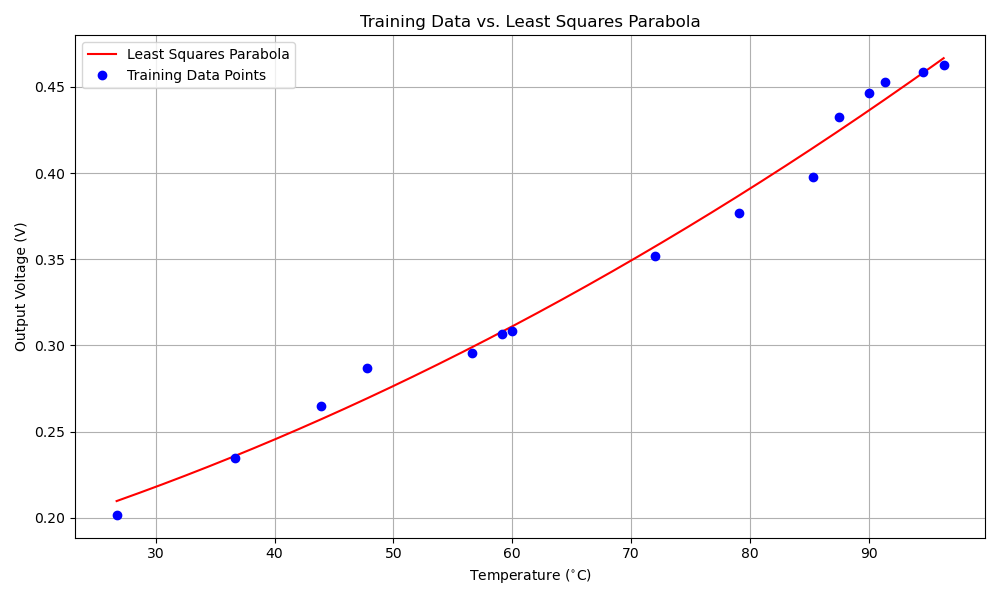
\includegraphics[width=0.9\columnwidth]{figs/training_data.png}
    \caption{Training data points plotted against the fitted Least Squares parabola.}
    \label{fig:training_plot}
\end{figure}

\subsection{Model Validation}
The accuracy of the trained model was verified using a separate validation dataset (Table \ref{table:validation_data}) that was not used during training. The model's predictions for the validation data points were compared against their true temperature values. The results, shown in Table \ref{table:validation_results}, indicate a close agreement between predicted and actual temperatures, confirming the model's validity. The graphical representation of this validation is shown in Fig. \ref{fig:validation_plot}.

\begin{table}[!h]
  \centering
  \caption{Validation Data: Temperature vs. Voltage}
  \label{table:validation_data}
  \begin{tabular}{|c|c|}
    \hline
    \textbf{Temp ($^{\circ}$C)} & \textbf{Voltage (V)} \\
    \hline
    36.8 & 0.23571 \\
    93.1 & 0.45391 \\
    57.3 & 0.29921 \\
    73.4 & 0.35621 \\
    \hline
\end{tabular}

\end{table}

\begin{table}[!h]
  \centering
  \caption{Validation Results}
  \label{table:validation_results}
  \begin{tabular}{|c|c|c|}
    \hline
    \textbf{Actual Temp ($^{\circ}$C)} & \textbf{Voltage (V)} & \textbf{Predicted Temp ($^{\circ}$C)} \\
    \hline
    36.8 & 0.23571 & 36.64 \\
    \hline
    93.1 & 0.45391 & 92.83 \\
    \hline
    57.3 & 0.29921 & 57.17 \\
    \hline
    73.4 & 0.35621 & 73.20 \\
    \hline
\end{tabular}

\end{table}

\begin{figure}[!h]
    \centering
    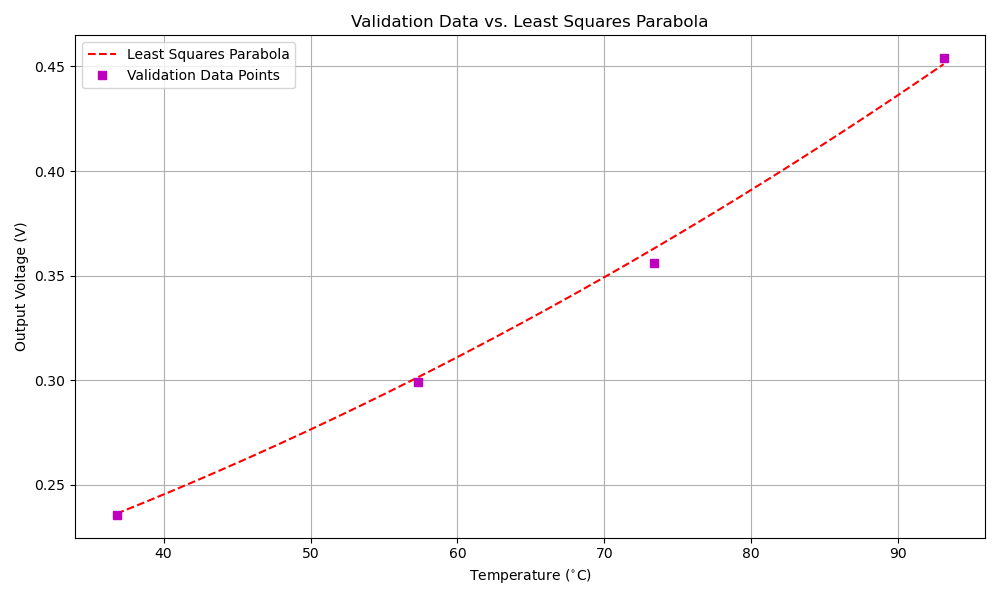
\includegraphics[width=0.9\columnwidth]{figs/validation_data.png}
    \caption{Validation data points plotted against the model's predictive curve.}
    \label{fig:validation_plot}
\end{figure}
\newpage

\section{Conclusion}
This project successfully demonstrates the construction and calibration of a high-precision temperature sensor. The use of a quadratic model derived from a Least Squares fit proved to be an effective method for converting raw voltage data into accurate temperature readings. The model's performance was successfully verified against an independent validation dataset, confirming its reliability. However, it was noted that the noise in power input has caused discrepencies in readings, which can be avoided by using as instrumentation amplifier before being connected to the ADS1115 module, to cancel out the noise.

\end{document}
